\documentclass{report}
\usepackage{url}
\usepackage{graphicx}
\usepackage[top=1in, bottom=1.25in, left=1.0in, right=1.0in]{geometry}
\usepackage{titlepic}

\title{AG DSN NAT Gateway Concept}

\date{February 28, 2017}
\author{Felix Kluge \and Simon Hanisch}
\titlepic{
\includegraphics[width=0.70\textwidth]{../agdsn_logo_quadratisch.pdf}}

\begin{document}

\maketitle
\tableofcontents

\chapter{Introduction}\label{introduction}

\section{Motivation}\label{motivation}

The network connections in the local residential homes currently suffer
from a simple but substantial problem: only IPv4 addresses are provided
by the university and there are only enough addresses to assign one to
each student. The fact that everybody owns more than one IP address capable device
today leads to the need of network address translation (NAT). The situation right now is that
every student needs to buy a small router that performs the NAT for him. This solution works
in the current setup but interferes with our plans to provide infrastructure WLAN for our users.
With infrastructure WLAN the user no longer connects to his own private network, meaning that his router can no longer
perform the NAT for him. The NAT has to be provided by the AG DSN. Another side effect
of this is that the user no longer needs to buy a router, which leads to less wireless networks 
interfering with our infrastructure WLAN. The goal of this project is to build a central NAT solution
for all our users.

\section{Nomenclature}\label{nomenclature}

\paragraph{Network Address Translation (NAT)}

Network Address Translation is the process of exchanging the address
information of a network packet. It is often required, because there are
not enough public IPv4 addresses for all hosts of a network. A private
network is used for those hosts and the internal IP addresses get
translated by a NAT gateway before the packet leaves the network. The
gateway tracks the connection of each host in the network to the public
network and thereby the internal host that needs to receive the related
incoming traffic from the public network.

\paragraph{Source NAT (SNAT)}

The source IP address gets exchanged by the gateway, this is the normal
NAT mode in use by consumer routers.

\paragraph{Destination NAT (DNAT)}

Destination NAT is required if a service localed on an internal host should be available on
the public network. When the gateway receives traffic from the public
network on a specific port the traffic is forwarded to the host (usually
known as port forwarding in customer routers). So the destination
address of a packet gets changed without the internal host creating a
connection first.

\paragraph{Classless Inter-Domain Routing (CIDR)}

The term Classless Inter-Domain Routing describes an approach to optimize
the usage of the 32 bit IPv4 address space. It is used in this document
to describe subnets and their size.

\section{Features}\label{features}

\subsection{Private Networks}\label{private-networks}

Every user of the network gets a private network (also
referred to as ``home network''). The term ``network'' refers to a VLAN
according to IEEE 802.1Q\cite{802.1Q}. This network will be located at the router
next to the users flat. If the user tries to connect to the network via
LAN or WLAN inside his building, he will be placed inside this network. This
implies that all entirety networks are only distinct inside the building,
not in a global (whole of residential homes) context. The IPs assigned inside a private network are
going to be RFC6598 addresses\cite{CGN}, in practice an /24 network out of the
Carrier-Grade NAT (CGN) range (100.64.0.0/10). Every private network
will be mapped via network address translation (NAT\cite{NAT}) to an external IP
address on the NAT gateway. Every external IP address is only in use by a single user.


\subsection{Roaming Networks}\label{roaming-networks}

All buildings get a unique network (VLAN) for roaming purposes. When a user connects to the network
at another building, i.e. not where his flat is located, he is placed inside
this local roaming network. These networks will contain an subnet from
the CGN allocation. Per default, connections from roaming networks are
not translated to external IP addresses. As a result, no connectivity to
addresses outside of the internal network is possible. During the
authorization of a client in an roaming network, a rule is created on
the NAT gateway. This rule translates connections to the assigned
private IP address to the public IP address of the user. Another approach to solve these
roaming issues is IP mobility as described in RFC3344\cite{IPMob}. It is described in the chapter IP Mobility \ref{ip-mobility}.



\subsection{Rate Limiting}\label{rate-limiting}

Due to an agreement with the university, the network connection for
individual users must be limited if a certain amount of traffic is
exceeded. Instead of blocking the access to the network for those users,
rate limiting will be performed by the NAT gateway. It is possible to 
configure exceptions, for certain destinations, that are excluded from the rate limiting.


\subsection{Failover}\label{failover}

The setup allows multiple NAT gateways to provide high availability. If one
gateway fails, the network stays operational. To achieve failover,
the connection state needs to be synchronized. The tool to synchronize
the connection tracking state between multiple hosts running linux (see Setup \ref{live-setup} chapter for details) is
conntrackd\cite{conntrack-tools}. Besides the connection tracking state, the availability
of the gateways is ensured by using keepalived\cite{keepalived}, a VRRP daemon for Linux.
For failover, multiple setups are possible.

\paragraph{Active - Passive}

Only one gateway is active, the other one is passive and becomes active
if the other gateway fails. This setup is easy to set up but wastes
resources, because one gateway is idling.

\paragraph{Active - Active (Synchronous Routing)}

The internal hosts are split up into two sets and each gateway gets to
perform NAT for one set. So both gateways are active and can be used as
backup for the other gateway. The load balancing in this case is static
and can be performed with policy based routing. Both directions of a
connection get translated by the same gateway (Synchronous Routing).

\paragraph{Active - Active (Asynchronous Routing)}

This is the most complex setup, because it is not clear which gateway
performs the translation. This is why the connection tracking state has
to be synchronized continuously and with a very low latency.
Example: A request by an internal host is translated by gateway X and the response
is translated by gateway Y. During the time the response needs to
arrive, the connection tracking state has to be synchronized -- otherwise,
the packets are rejected. This scenario allows dynamic load balancing
between multiple NAT gateways without knowledge which gateway a packet is processed on.


\subsection{Port Forwarding}\label{port-forwarding}

NAT prevents users to use remotely initiated connections. To address
this issue, port forwardings are configurable. In detail, the NAT
gateway allows incoming connections to the external (``public'') IP addresses
and forward them to an configured internal host inside a private
network. Related to port forwarding, a feature set comparable to
publicly sold routers is available. Popular examples are TP-Link
routers (e.g.~TL-WR841ND\cite{TL-WR}) and AVM routers (e.g.~Fritzbox 4020\cite{fritzbox}), which
allow the user to configure forwarding rules. Criteria for these rules are the
inbound (external) port and the protocol. The redirection is possible to
an configurable internal IP address and port.

\subsection{Internal API}\label{internal-api}

To set up the NAT gateway, an interface to the configuration tools already in
place is required. This targets the user management tool and the user
self-service tool. In addition, the DHCP server for roaming
networks needs to be able to perform updates on the NAT gateway. These
other parts of the infrastructure are not part of this project, but the
interface of the gateway should be designed for their needs.

\chapter{Basics}\label{basics}

\section{IP Mobility}\label{ip-mobility}

IP mobility\cite{IPMob}\cite{MobileIP-cisco} uses a complex setup to allow roaming users to retain an
IP address from their home network. An endpoint in the home network of the
user - called the home agent - forwards traffic for the user to his real
point of presence in the network, the so-called foreign agent. The
foreign agent establishes a tunnel to the home agent, using its own IP address
as a care-of address for the roaming user. All traffic for the client IP address in the home network
can now be forwarded in a tunnel to the foreign agents IP address. The client
itself is bound to an address of the subnet at his point of presence.

\paragraph{Advantages}\label{pro}

\begin{itemize}
\itemsep1pt\parskip0pt\parsep0pt
\item
  No dynamical NAT configuration necessary
\item
  L2 connectivity to the home network (e.g.~printers)
\end{itemize}

\subsubsection{Disadvantages}\label{con}

\begin{itemize}
\itemsep1pt\parskip0pt\parsep0pt
\item
  Home- and foreign agents for every network necessary (costly)
\item
  traffic is encapsulated (overhead)
\end{itemize}

\paragraph{Aruba IP Mobility}\label{aruba-ip-mobility}

The wireless network equipment vendor Aruba offers a Mobile IP
implementation for his wireless equipment \cite[p. 659]{MobileIP-Aruba}. The wireless
controllers are used as agents. However, relying only on this commercial
solution leads to several different disadvantages:

\begin{itemize}
\itemsep1pt\parskip0pt\parsep0pt
\item
  Roaming is only available in buildings with a WLAN controller
\item
  Each residental home needs a WLAN controller (costly)
\item
  It is unknown if the solution is technical applicable to our environment
\item
  The whole setup is locked down to Aruba
\end{itemize}

The technical issues will be investigated in the future. The reason it may not
work in our environment is due to the determination of the home agent in the network.
According to the documentation the calculation is based on the user VLAN IP subnet \cite[p. 661]{MobileIP-Aruba}.
To work properly in our network, VLAN ids may not be unique in the whole network.


\section{Netfilter Hooks}\label{netfilter-hooks}

The netfilter hooks\cite{hooks} allow to tap into the network traffic on a linux
machine in specific places in the network stack. The different hooks
allow to access the network traffic in specific stages, making filtering,
altering and analysing pretty flexible. Figure \ref{Hooks.pdf} shows an overview of the different hooks in the network stack.
The important hooks for NAT are PREROUTING and
POSTROUTING. For source NAT the destination IP address has to be correct in order to change the source IP address correctly. For destination NAT
it is the other way round. It must be performed before the routing,
otherwise its not clear what the actual destination IP address is and how the packet has to be routed.

\begin{figure}[ht]
	\centering
	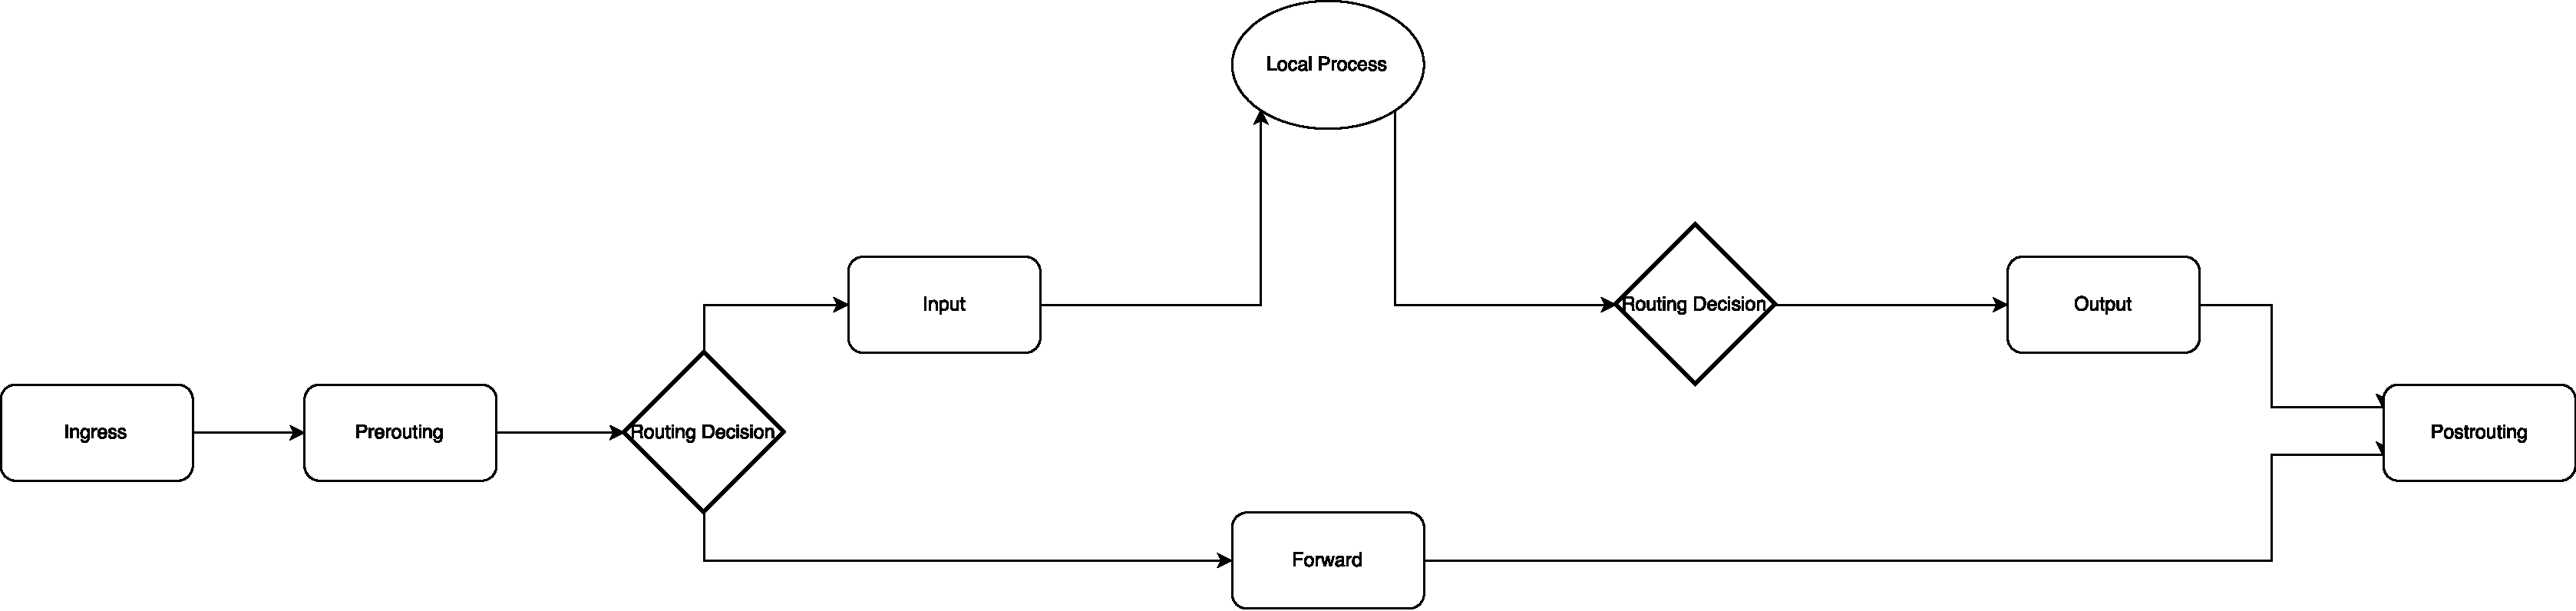
\includegraphics[width=\textwidth]{../Hooks.pdf}
	\label{Hooks.pdf}
	\caption{netfilter hooks}  
\end{figure}

\chapter{Management Component}\label{management-component}

\section{Structure}\label{structure}

The management component is a python3 celery application. Celery is a
framework designed for asynchronous task queue execution\cite{celery}. It
enables management components in the network to trigger
configuration changes at the gateway. Updates are distributed by a rabbitmq message
broker\cite{rabbit}. An example configuration for the management component
can be found in the appendix at \ref{celery-application}.


\section{Data Model}\label{data-model}

\subsection{Translations}\label{translations}

Translations are used to configure NAT mappings. They contain the public
IP address and the private subnet. Private subnets do not have a fixed size.
This design allows single forwarding entries for roaming users represented by
private subnets as small as a singe host (/32). Home networks with an expected
size of 254 hosts (/24) can be represented in these objects, too.

\subsection{Forwardings}\label{forwardings}

These objects are used for DNAT to allow incoming connections to users.
They contain the following data: public IP address, private IP address, protocol, source
port and destination port.

\subsection{Throttles}\label{throttles}

Throttle objects are used to describe limited connections. They contain
the private network or host, the public IP address and the limiting speed in
kbytes/second. Public and private addresses are both required, because
inbound and outbound connections have to be limited. The speed limit is
shared for inbound and outbound connections as the same queue is used.

\section{Program State}\label{program-state}

The application supports two ways to update its configuration.

First, a task named initialization is possible. It is called after
the start of the application. During the initialization, the first
configured database is queried to generate a complete ruleset. The
conntrack state of the NAT gateway for the configured private network range is
dropped. Nftables configuration on all relevant tables is dropped and the
new state is applied. The initialization process can later be utilized
to reset the gateway.

Second, incremental state updates are possible. They are triggered by
the message broker with parameters to exactly identify the required
change. During an update, the relevant database is queried for the data.
The content of the change is not communicated via the message broker but
the database, so the broker only signals the application that an
update is required.

\section{State Updates}\label{state-updates}

As mentioned above, the application queries the database to determinate
which action to perform during a signalized state update. Two
scenarios are possible: the data may or may not be present in the
database.
If there is no matched data in the database, the application
assumes that the represented data (translation, forwarding or throttle)
has to be dropped from nftables configuration. Then it
performs the necessary tasks to delete the entries. This may include
dropping conntrack state information.
If matched data is inside the Tabaksdose, the application rewrites
all affected nftables rules. This may result in a newly created rule or
in an updated rule, depending on the object in question and the current
nftables state. For example, translations allow direct rule replacements.
An already present rule may be updated with the ``nft replace rule'' command.

\begin{figure}[ht]
	\centering
	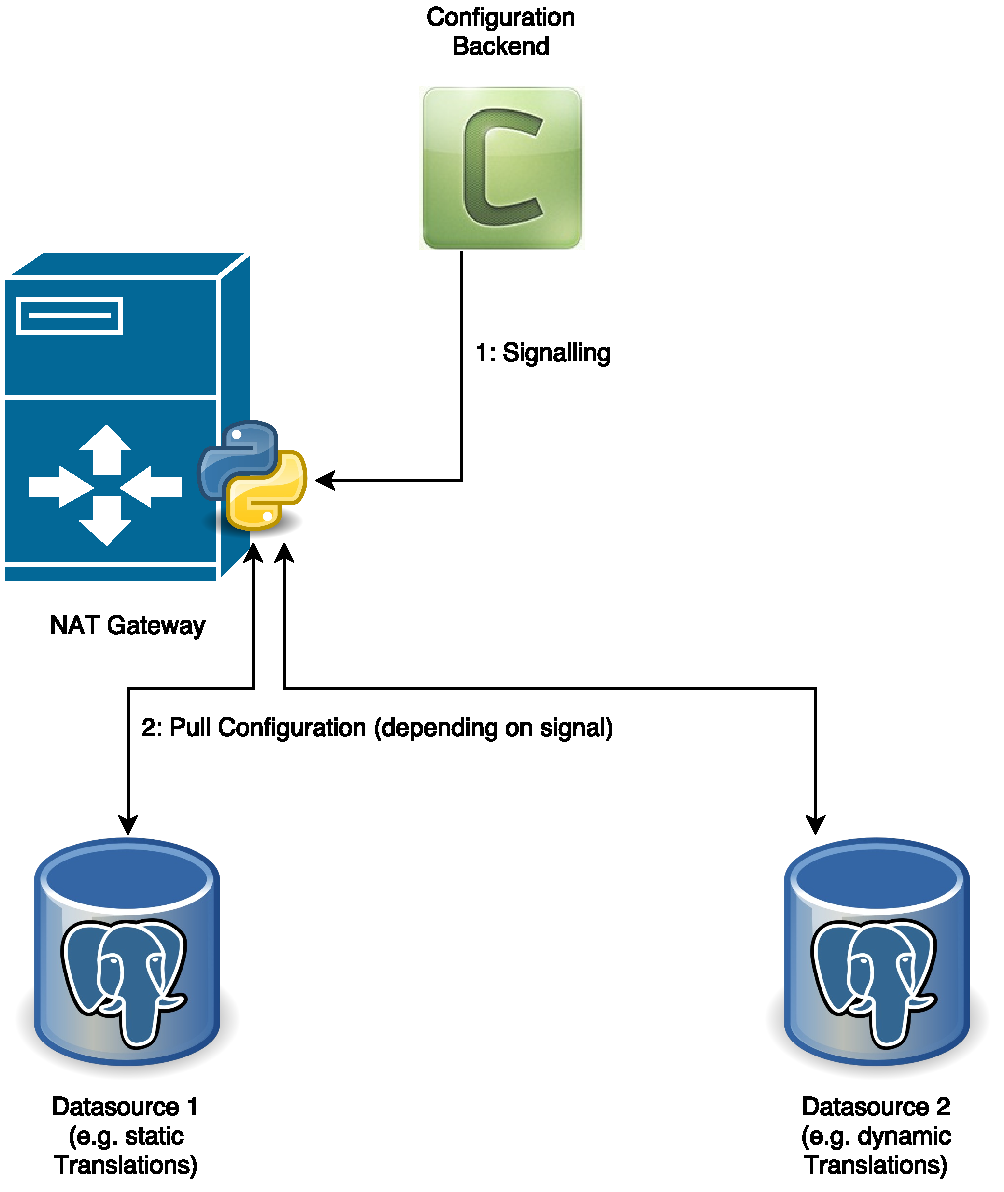
\includegraphics[width=0.60\textwidth]{../ApplicationDeployment.pdf}
	\label{ApplicationDeployment.png}
	\caption{State updates}  
\end{figure}

\chapter{Implementation}\label{implementation}

\section{packet filter}\label{packet-filter}

Packet filter (pf)\cite{pf}\cite{pfOpenBSD} is a firewall for the BSD-Family and was
original written for OpenBSD. Besides filtering pf is moreover able to perform NAT
and bandwidth control. Due to time issues we did not implement a
solution with pf, but evaluated some basic constrains. Instead of using
OpenBSD we would recommend using FreeBSD, because OpenBSDs PF is not able to
utilitise multi core processors \cite{pfOpenBSD}. This may causes performance issues,
so this feature may be important. Also the Solarflare network cards of our gateways are
only supported on FreeBSD. Like the other solutions pf keeps track of
connections and only traverses the NAT rule set if the packet does not
belong to an existing connection. For redundancy pf uses pfsync\cite{pfsync},
which allows the synchronization of state table entries between
multiple pf instances.

\section{pfSense}\label{pfsense}

An related project is pfSense\cite{pfsense}, a firewall distribution based on
OpenBSD and PF. The software includes an webinterface, is actively
maintained and has an online community. Sadly, it's not possible for us
to use this existing project, since it does not provide an API to do
remote configuration. This feature is planned for the 3rd release of
pfSense, but the release date is unknown until further notice.


\section{Iptables}\label{iptables}

iptables\cite{iptables} is the de facto standard for network packet manipulation on
Linux. It is a user-space application that allows configuration of
the packet filter ruleset in the Linux kernel. Besides filtering, it can
be used to perform NAT. There are different implementations of iptables
for different protocols like IPv6 and ARP. Iptables has 5 standard
tables: filter, nat, mangle, raw and security. Filter is the default
table and is used for filtering unwanted packets, it has the INPUT,
FORWARD and OUTPUT hooks registered. The nat table is for performing
NAT, packets pass this table only when a new connection is created. Its built-in
hooks are PREROUTING, OUTPUT and POSTROUTING. To alter
packets, the mangle table is used. Raw is for configuring exemptions to
the connection tracking and security is used for Mandatory Access
Control. Besides the standard tables, new tables can be added to perform
specific tasks. Tables contain a set of chains containing multiple rules.
Rules match traffic and then perform a specific task, like NAT or
jumping to another chain.

\section{Nftables}\label{nftables}

nftables\cite{nftables}\cite{nftables2}\cite{nftables3} is a new packet classification framework for Linux that aims to
replace iptables. It was first introduced on the netfilter workshop 2008
and got its first official release in 2009. Besides iptables, the tools
ip6tables, ebtables and arptables are going to be united in nftables.

The motivation behind this new tool is the age of iptables and many
problems like the representation of the ruleset as huge blob, which
makes replacement of single rules impossible. The ruleset is not very
memory efficient and can not be translated back into rules. Another
mayor drawback is that iptables, ip6tables, ebtables and arptables share
a large codebase but are not the same tool, which makes the code
management inefficient. Nftables also comes with an easier syntax and
allows multiple targets per rule, making rulesets less redundant. It is
also possible to exchange single rules in a ruleset without reloading
the entire table.

nftables consists of three main components: the kernel modules, nft (the
nftables user-space application) and libl the netfilter netlink library
for communication with the kernel.

The basic container in nftables is a table, it contains rules and chains
of the same protocol family. Chains are the containers for rules and can
be used as jump targets. A chain with a netfilter hook is
called a base chain and serves as entry point into a table. Rules are
container of expressions that define the runtime behavior and are the
smallest unit that can be replaced. Besides these basic building blocks,
nftables allows the usage of sets and maps. They make it easy to specify
rules without much redundancy working for the entire used data structure.
Especially maps are a useful addition for NAT, because they allow to
directly specify NAT mappings. There are two different implementations
for sets, rbtree or hashmap. Nftables internally decides which one its
going to use.

\section{Conntrack / Conntrackd}\label{conntrack-conntrackd}

Conntrack\cite{conntrack-tools} is a user-space application that provides access to the
connection tracking module\cite{conntrackSys} of the Linux kernel. The sole use of the
connection tracking module is to store information about connections
that pass the machine. Each connection is identified by the source and
destination IP addresses, the port numbers, and protocol type. The
connection tracking module stores information about the state of the
connection and is vital for NAT, because it allows to match incoming
traffic from the internet to internal hosts.

After the initial NAT through nftables or iptables, a conntrack entry gets
created in the connection table, containing the new source IP address.
All following packets of the same connection are directly translated
using the conntrack entry and do not pass through the nat table. \\

Example conntrack:


\begin{verbatim}
         icmp 1 4 src=100.64.0.10 dst=192.168.30.0 type=8  code=0 id=7224
         src=192.168.30.0 dst=192.168.0.19 type=0 code=0 id=7224 mark=0 use=1
\end{verbatim}

The first src, dst matches the original traffic from the internal host,
the second pair matches the response from the host on the other side of
the gateway. The conntrack contains all the information needed to
perform the NAT.

Conntracks can have different states:

\begin{itemize}
\item
  NEW: The connection is starting, to reach this the state the packets
  only have to be valid, no reply packets have been received yet.
\item
  ESTABLISHED: The connection is established, this means the gateway has
  seen replies to the connection.
\item
  RELATED: An expected connection, that is used for some special
  protocols like FTP. They are created by so called helpers that can
  extract information out of a connection that lets you expect another
  connection in the future. For example, the control flow for FTP is done
  over port 20, but the data connection is done with a different port
  that is sent to the client by the server. The ftp helper extracts that
  port number and sets up an expected connection for that port, allowing
  this connection to pass the NAT gateway.
\item
  INVALID: The connection does not follow valid network communication.
\end{itemize}

The Kernel module uses a hash table for efficient lookups, that holds 2
hash values for every connection: one for the original direction and another
for the reply direction. The hash contains all necessary information to
match the connection like the source and destination IP address. The two
hash values point to the conntrack that holds the state information of
the connection. Current connections are not altered during NAT rule updates.
Only new connections are immediatly affected by the rule changes. To change all
connections to a new IP address the old conntrack state needs to be dropped.

Besides the kernel module for conntrack and the user-space tool, there is the
daemon conntrackd. The daemon allows state table synchronization
between different NAT gateways. Utilising the state synchronization, it is
possible to setup fault tolerant NAT gateways that do not lose
connections in the case of an failure. In our setup an extra link
between the gateways is used to replicate state information with a low-latency.
This allows us to use asynchronous routing with our gateways, meaning that a
connection can be translated by one gateway in one
direction and translated back by the other gateway in the opposite
direction. We performed tests that suggest that this setup works, but we have
to wait for live tests to be sure. If it does not work,
we have to make sure that a connection passes the same gateway in both
directions (for example by splitting up the IP addresses for the
gateways).

The maximum size of the connection tracking table can be adjusted with
the variable \linebreak \textit{net.ipv4.netfilter.ip\_conntrack\_max} and should be
increased from the default value. Conntrackd also has an option specifing
the maximum number of conntracks.

\section{Keepalived}\label{keepalived}

Keepalived\cite{keepalived} is a Virtual Router Redundancy Protocol (VRRP)\cite{vrrp} deamon
for Linux. Its main goal is providing simple loadbalancing and
high-availability for routers and servers running Linux. VRRP allows to
configure one virtual router with an IP address using a set of hardware
routers. The virtual IP address gets assigned to a specific hardware router by
VRRP, making this router the VRRP master. The other routers
function as backup routers for the master. If the master fails, the VRRP
assigns the IP address to a new hardware router. This functionality allows easy
fail over for routers and servers.

In our setup both gateways are active at the same time, making it
necessary to configure two virtual gateways, each gateway
providing backup functionality for the other. We added the configuration file
we used for our evaluation scenario in the appendix at \ref{conntrackd.conf}.


\chapter{Setup}\label{setup}

\section{Live-Setup}\label{live-setup}

The central router in our network is called Ianus and connects to
our uplink. Ianus consists of two hardware routers located at different
buildings. To ensure availability, one NAT gateway will be located at
each of those locations. Each gateway will be connected to both hardware
routers of Ianus. This ensures availability in case that one gateway or
one hardware router fails.

All outgoing user traffic will be sent to the gateways and from the
gateways back to ianus. Through this loop setup it is very easy to not
route traffic over the gateways that should not be translated (e.g.
connections to and from our servers).


\begin{figure}[ht]
	\centering
	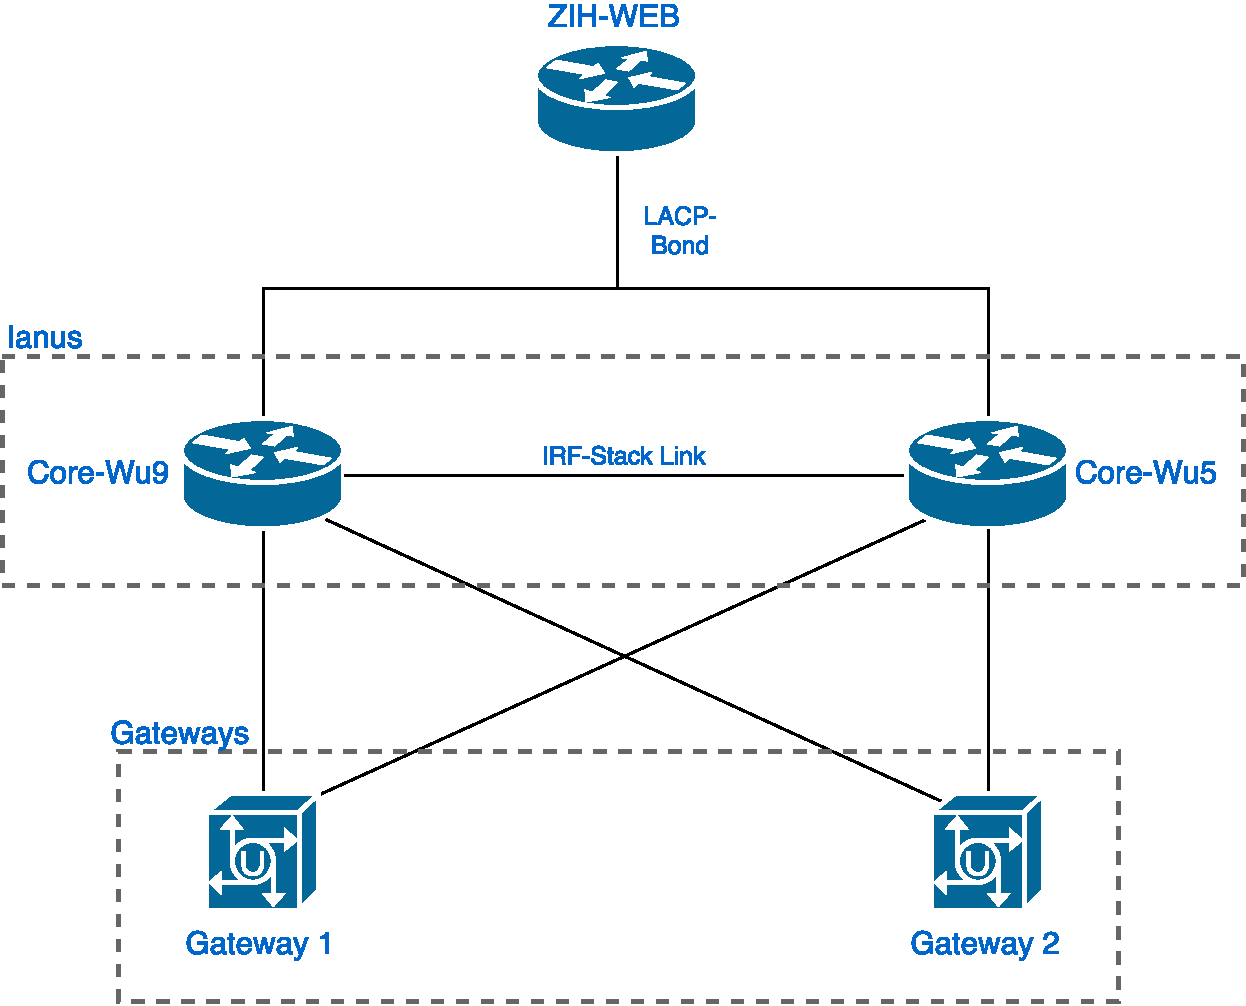
\includegraphics[width=\textwidth]{../LiveSetup.pdf}
	\label{LiveSetup.pdf}
	\caption{The live-setup with the connections between the gateways and Ianus}  
\end{figure}

\begin{figure}[ht]
	\centering
	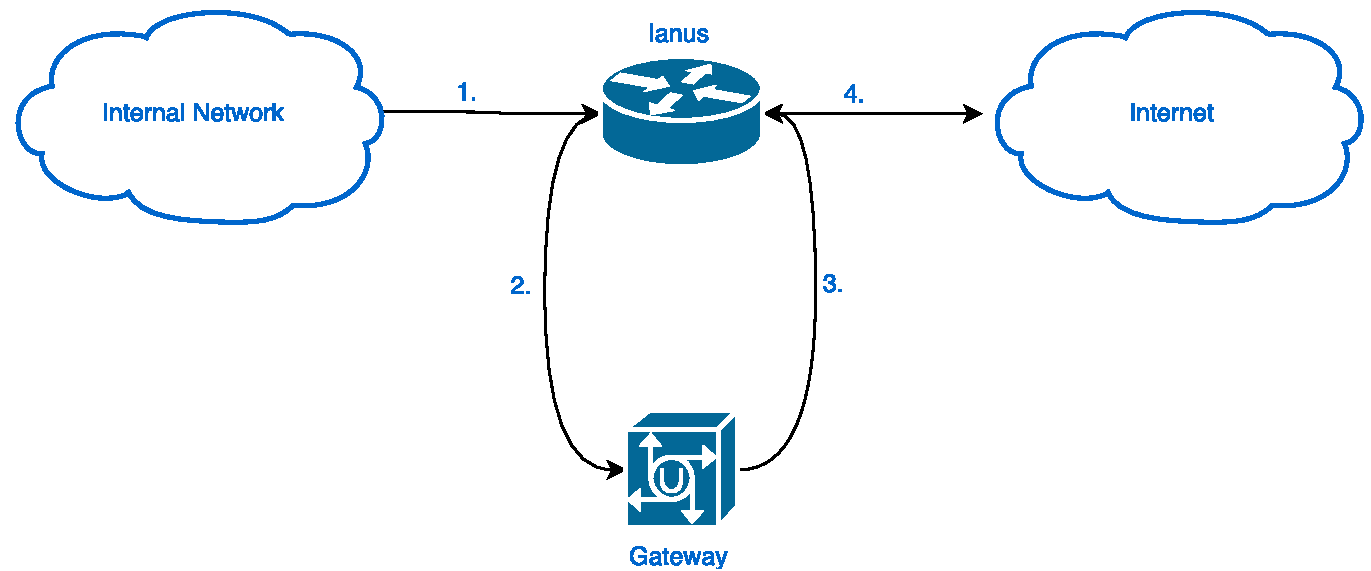
\includegraphics[width=\textwidth]{../NetworkFlow.pdf}
	\label{NetworkFlow.pdf}
	\caption{This is the normal traffic flow for an internal host that communicates with the internet}  
\end{figure}


\section{Gateways}\label{gateways}

The general hardware/software specifications for our two NAT gateways (Dell PowerEdge R630 Server): \\
\begin{description}
\item CPU: 2x Intel Xeon E5-2690 v4 (2,6GHz, 14 Cores/28 Threads)
\item RAM: 2x 16GB RDIMM 2.400MT/s
\item first NIC: Intel Ethernet i350 4 Ports 1GbE
\item second NIC: 2x Solarflare Flareon Ultra SFN8522 10 Gigabit SFP+
\item harddrive: 200GB SSD
\item OS: Debian stretch, Kernel \textgreater{}= 4.8
\item nft: \textgreater{} 0.7 (build from the git repo)
\end{description}

\chapter{Evaluation}\label{evaluation}

\section{Introduction}\label{introduction-1}

To check if the NAT gateway is capable of serving all our users, we
relied on performance/stress testing to see what the gateway is capable
of. Generating adequate amounts of network traffic for testing was challenging.
Traffic can vary on different characteristics: used protocols, bandwidth, packet amount,
packet length and connections.

A simple test with iPerf\cite{iperf} revealed that pure bandwidth had little
to no effect on the NAT gateway. Another test with a few million
packets per second showed the same. Only when we started using more
connections (different source ip address destination ip address pairs), the cpu usage on
the NAT gateway went up. This is because only the first packet of a
network connection traverses the NAT rules in nftables or iptables. All
following packets are directly processed by the connection tracking
system of the kernel. Based on this conclusion, our stress testing relies on creating
as many connections as possible.

The problem with connections is that they can not be generated as easy as
lots of packets or bandwidth. Mostly because there needs to be an
response to a request that traverses the NAT gateway in the opposite
direction. This makes techniques like IP-spoofing impractical. All
IP addresses in use need to be configured on the corresponding machines (now is
a good time to increase the size of your ARP cache).

\section{Setup}\label{setup-1}

In Figure \ref{EvaluationSetup.pdf} you can see our setup. We used one virtual machine to simulate
hosts in ``The Internet'' (192.168.0.0/16) and one for our home networks
in the Carrier-grade NAT (CGN)(100.64.0.0/12). For ``The Internet'', the
NAT gateways have all public IP addresses configured that are used for
NAT (of course not both gateways at the same time). In the Carrier-grade
NAT each gateway only needs one IP. Between the two gateways there is a
link for state synchronization of the conntrack tables.

An internal host, simulated by the ``Home Networks'' vm, sends a packet
over one of the gateways to an internet host. After the first packet has
traversed the NAT rules, a conntrack is created and synchronized with the
second gateway. The internet host receives the packet and sends a
response via the gateway that has the corresponding IP address
configured. The gateway then forwards the message to the internal host.

\begin{figure}[ht]
	\centering
	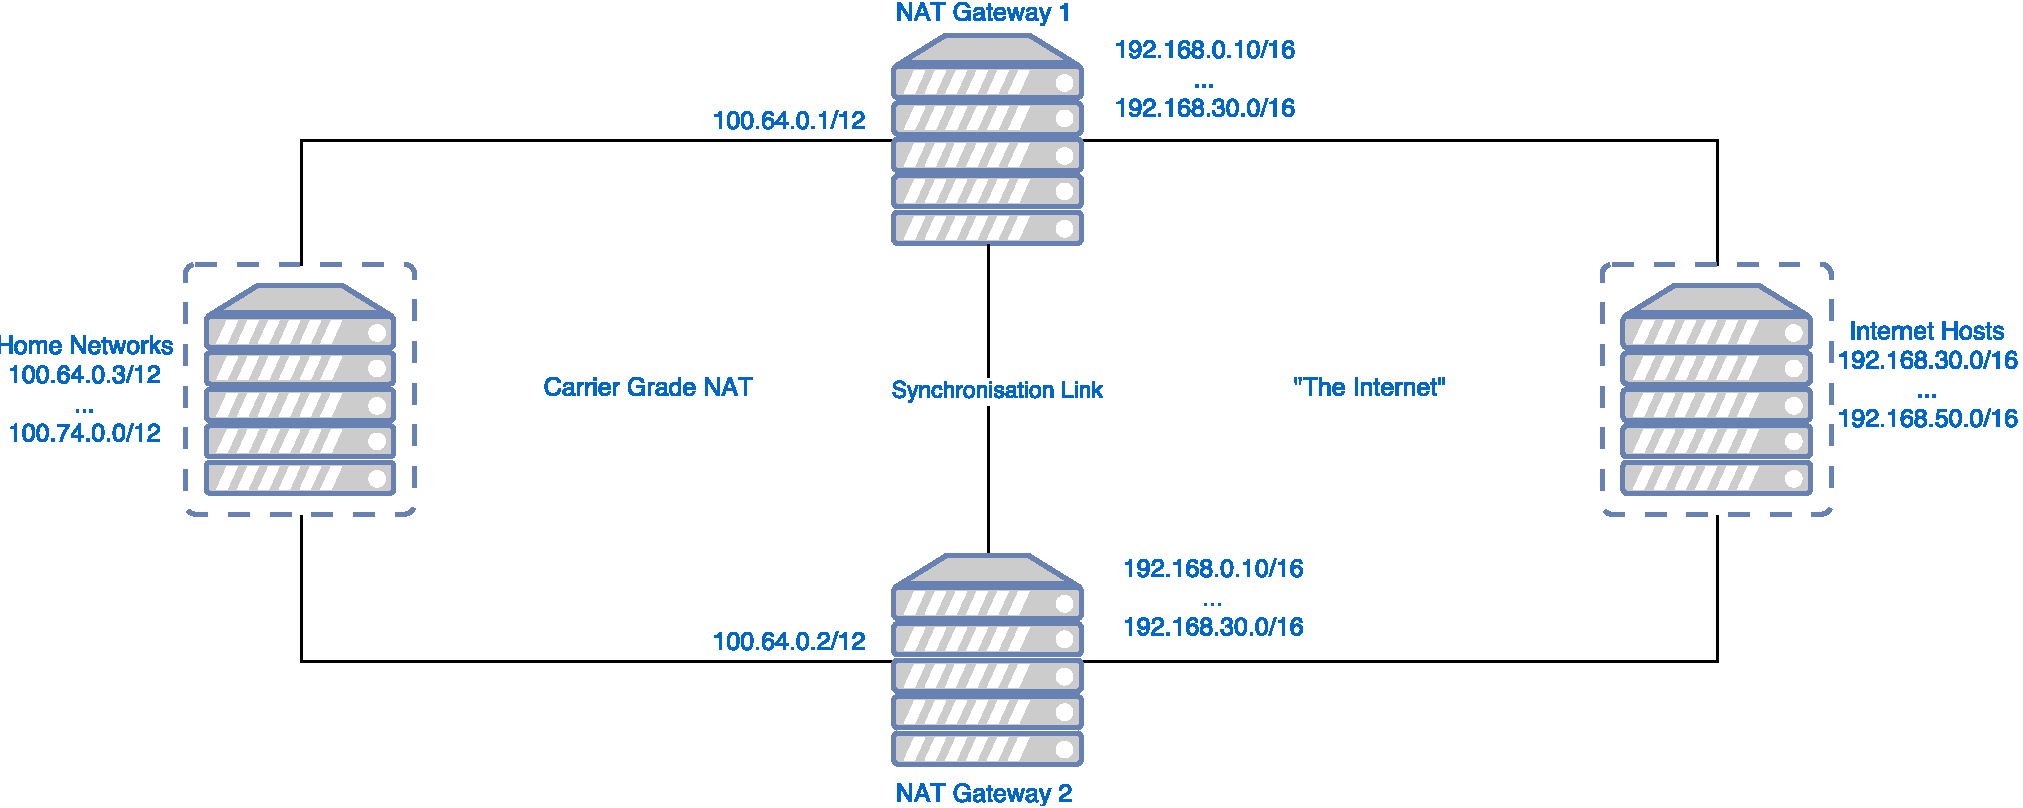
\includegraphics[width=\textwidth]{../EvaluationSetup.pdf}
	\label{EvaluationSetup.pdf}
	\caption{Evaluation setup}  
\end{figure}

\section{Generating Traffic}\label{generating-traffic}

After some initial testing with packet generation tools and python, we
had problems generating network traffic that puts much load on the
machines. The key to generating good workload is to generate lots of
different connections, meaning lots of different source IP and destination
IP pairs. To generate them easily we found the unix tool nping\cite{nping}
very helpful. Nping is part of nmap\cite{nmap} and supports multiple target
IPs (up to 8900) and gives you a lot of control about how the packets
are generated. It supports TCP, UDP and ICMP packet generation and can
use a specified source IP address, port and interface. The payload of
the nping packets can be specified as well. This feature set makes nping
an excellent tool for our use case.

To generate more connections, we started multiple instances of nping with
different source IP addresses. We will include the used python script in
the appendix.



\section{Metrics}\label{metrics}

The metrics we are interested in are latency, resource consumption on
the gateway and the synchronization of conntracks. All of them together
should help us to find bottle necks and identify problems in the
gateways.

The latency is interesting because it should be as low as possible to
not harm the hosts that are behind the NAT. We measured the latency by
using ping\cite{ping} from the internal hosts VM to the Internet Hosts VM.
To measure the resource consumption we used collectl\cite{collectl}, a unix tool that
can measure various resources on a pc. We used it to measure the cpu
utilization, network traffic and interrupts on the gateways. The polling
interval was one second. For the synchronization of the state tables we
used ``conntrackd -s'' and polled this statistic every second with a
script. Another metric we looked at was the memory consumption, but we
could not find anything interesting here, so we excluded it.

\section{Results}\label{results}

Coming soon to an email server of your choice\ldots{}

\chapter{Appendix}\label{appendix}

\section{keepalived.conf}\label{keepalived-1}

\begingroup
\fontsize{9pt}{9pt}\selectfont
\begin{verbatim}
    global_defs {
        # Name of the local router
            router_id       chomsky

            # The email server
            smtp_server     192.168.0.30

        # Where to send notifications if a machine is down
            notification_email {
                    test@test.de
            }
    }


    # Groups of vrrp_instances that failover together, allows to call
    # scripts and send notifications 
    vrrp_sync_group agdsn_nat_1 {
            group {
                    cgn_1
                    ext_1
            }

            smtp_alert
            global_tracking
    }

    # Describes moveable IPs, sets the priority for the machine
    vrrp_instance cgn_1 {
            state           BACKUP

            interface       eth7

            virtual_router_id 10

            priority        150

            virtual_ipaddress {
                    100.64.0.1/12
            }
    }

    vrrp_instance cgn_2 {
            state           BACKUP

            interface       eth7

            virtual_router_id 11

            priority        100

            virtual_ipaddress {
                    100.64.0.2/12
            }
    }

    vrrp_instance ext_1 {
            state           BACKUP

            interface       eth6

            virtual_router_id 12

            priority        150

            virtual_ipaddress {
                    192.168.0.1/16
            }
    }

    vrrp_instance ext_2 {
            state           BACKUP

            interface       eth6

            virtual_router_id 13

            priority        100

            virtual_ipaddress {
                    192.168.0.2/16
            }
    }
\end{verbatim}
\endgroup

\section{nping}\label{nping}

\subsection{Example usage}

\begingroup
\fontsize{9pt}{9pt}\selectfont
\begin{verbatim}
Example usage:
nping -c 0 --tcp -p 80-1080 --interface eth1 -S 100.64.0.10 -g 5000 --rate 6000 <list of dest ips>

-c                -> Number of repeats, 0 is for infinity
--tcp             -> Probe mode
-p 80-1080        -> destination port, or port range
--interface eth1  -> the interface to use
-src              -> the source ip address of the interface to use (if there are multiple)
-g                -> the src port to use
--rate 6000       -> the packets per minute
\end{verbatim}
\endgroup

\subsection{Python script}

\begingroup
\fontsize{9pt}{9pt}\selectfont
\begin{verbatim}
import ipaddress
from subprocess import call


IP = ipaddress.ip_address('192.168.30.0')

dest_ips = ""
for i in range(8900):
        dest_ips += str(IP) + " "
        IP += 1

SRC_IP = ipaddress.ip_address("100.64.0.10")

call("date", shell=True)

for i in range(30):
        call("nping -c 0 --tcp --interface eth1 -S " + str(SRC_IP) + " -g "
        	+ str(5000 + i) + " --rate 6000 " + dest_ips + ">> /dev/null &", shell=True)
        SRC_IP += 256
\end{verbatim}
\endgroup

\section{nftables}\label{nftables-1}

\subsection{map}

This is a simple Map config for nftables. We wanted to use Maps for our
solution but found that they are still to buggy to be used in a live setup.
We hope to utilize them in the future, since they are simpler than building
a tree. Maps use a RBTree internally so the complexity is still
log(n) like in our other solution. The issues we had so far with maps:

\begin{itemize}
\itemsep1pt\parskip0pt\parsep0pt
\item
  Adding new elements to a map had a memory leak (this was fixed by the
  maintainer)
\item
  Very high memory consumption when updating a map entry
\item
  Only the first two rules in a map worked (the maintainer send us a
  patch for the kernel module but we still have to try it)
\item
  Deleting elements of the map is currently not possible.
\end{itemize}

\begingroup
\fontsize{9pt}{9pt}\selectfont
\begin{verbatim}
#!/usr/sbin/nft
add chain nat postrouting { type nat hook postrouting priority 100 ;}
add chain nat prerouting { type nat hook prerouting priority 0 ;}
add map nat subnettoip { type ipv4_addr: ipv4_addr ; flags interval ; }
add rule ip nat postrouting snat ip saddr map @subnettoip;
add element nat subnettoip { 100.64.0.0/24 : 192.168.0.19 }
add element nat subnettoip { 100.64.1.0/24 : 192.168.0.20 }
add element nat subnettoip { 100.64.2.0/24 : 192.168.0.21 }
add element nat subnettoip { 100.64.3.0/24 : 192.168.0.22 }
\end{verbatim}
\endgroup

\subsection{tree}

We have up to 6000 /24 Networks that we want to NAT to specific IP addresses.
Simply adding them all in one chain would be to slow, that is why we
created a tree of chains. Starting with 2 networks at the top and than 8
networks per level. In the leaf chain the actual NAT rule is defined.
Below is the start of our tree config for nftables down to the first 2
blocks of NAT rules. The rest of the tree is structured the same.

\begingroup
\fontsize{9pt}{9pt}\selectfont
\begin{verbatim}
#!/usr/sbin/nft
add table nat
add chain nat prerouting { type nat hook prerouting priority 0 ;}
add chain nat postrouting { type nat hook postrouting priority 0 ;}
add chain nat postrouting-level-0
add rule nat postrouting ip saddr 100.64.0.0/12 goto postrouting-level-0
add chain nat postrouting-level-0-0
add rule nat postrouting-level-0 ip saddr 100.64.0.0/15 goto postrouting-level-0-0
add chain nat postrouting-level-0-0-0
add rule nat postrouting-level-0-0 ip saddr 100.64.0.0/18 goto postrouting-level-0-0-0
add chain nat postrouting-level-0-0-0-0
add rule nat postrouting-level-0-0-0 ip saddr 100.64.0.0/21 goto postrouting-level-0-0-0-0
add rule nat postrouting-level-0-0-0-0 ip saddr 100.64.0.0/24 snat 192.168.0.19
add rule nat postrouting-level-0-0-0-0 ip saddr 100.64.1.0/24 snat 192.168.0.20
add rule nat postrouting-level-0-0-0-0 ip saddr 100.64.2.0/24 snat 192.168.0.21
add rule nat postrouting-level-0-0-0-0 ip saddr 100.64.3.0/24 snat 192.168.0.22
add rule nat postrouting-level-0-0-0-0 ip saddr 100.64.4.0/24 snat 192.168.0.23
add rule nat postrouting-level-0-0-0-0 ip saddr 100.64.5.0/24 snat 192.168.0.24
add rule nat postrouting-level-0-0-0-0 ip saddr 100.64.6.0/24 snat 192.168.0.25
add rule nat postrouting-level-0-0-0-0 ip saddr 100.64.7.0/24 snat 192.168.0.26
add chain nat postrouting-level-0-0-0-1
add rule nat postrouting-level-0-0-0 ip saddr 100.64.8.0/21 goto postrouting-level-0-0-0-1
add rule nat postrouting-level-0-0-0-1 ip saddr 100.64.8.0/24 snat 192.168.0.27
add rule nat postrouting-level-0-0-0-1 ip saddr 100.64.9.0/24 snat 192.168.0.28
add rule nat postrouting-level-0-0-0-1 ip saddr 100.64.10.0/24 snat 192.168.0.29
add rule nat postrouting-level-0-0-0-1 ip saddr 100.64.11.0/24 snat 192.168.0.30
add rule nat postrouting-level-0-0-0-1 ip saddr 100.64.12.0/24 snat 192.168.0.31
add rule nat postrouting-level-0-0-0-1 ip saddr 100.64.13.0/24 snat 192.168.0.32
add rule nat postrouting-level-0-0-0-1 ip saddr 100.64.14.0/24 snat 192.168.0.33
add rule nat postrouting-level-0-0-0-1 ip saddr 100.64.15.0/24 snat 192.168.0.34
\end{verbatim}
\endgroup

\subsection{HowTo}

This is a short collection of useful nftables commands we used during
our work.

Useful to know:

\begin{itemize}
\item
  If you use the type ``nat'' for a hook than only the first packet of
  each connection is processed by the chain
\item
  For NAT there always have to be chains with the prerouting and
  postrouting hook. For source NAT the prerouting chain is empty but
  still needed!
\item
  Jump returns to the calling chain after completion, goto never
  returns.
\item
  If a rate limit rule gets exhausted, the next rule in the chain is
  called, or the default policy applies. If a host should be throttled,
  all traffic that exhausts the rate limit needs to be dropped.

\end{itemize}

\begingroup
\fontsize{9pt}{9pt}\selectfont
\begin{verbatim}

# Adds the table nat to nftables
nft add table nat

# List the content of the table nat
nft list table nat

# List all tables in nftables
nft list tables

# Can also be used to make a backup of the ruleset
nft list table nat > backup.ruleset

# Load the ruleset backup.ruleset into nftables, see the tree config for an example config
nft -f backup.ruleset

# Deletes the table nat
nft delete table nat

# Deletes all rules in the table nat, chains are preserved
nft flush table nat

# Adds the chain prerouting to the table nat. The chain has the type nat
# and uses the prerouting hook with priority 0. Priority 0 means the its first.
nft add chain nat prerouting { type nat hook prerouting priority 0 \; }

# Add the chain postrouting to the table nat
nft add chain nat postrouting { type nat hook postrouting priority 100 \; }

# Deletes the chain postrouting in the table nat
nft delete chain nat postrouting

# Add a rule to the postrouting chain in the table nat. If the source ip address
# is in the network 100.64.0.0/15 goto chain targetChain
add rule nat postrouting ip saddr 100.64.0.0/15 goto targetChain

# Adds a snat rule to the chain postrouting in the table nat. All source ips from
# 100.95.255.0/24 of the interface eth0 get translated to 141.30.233.255
nft add rule nat postrouting ip saddr 100.95.255.0/24 oif eth0 snat 141.30.233.255

# Addes a rule to the input chain in the table filter. Rate limits the traffic 
# to 10 mbytes/second and accepts the traffic. When the rate limit is exhausted 
# the next rule is applied. If you want to throttle a host then a drop rule is needed.
nft add rule filter input limit rate 10 mbytes/second accept

# Adds a new named map subnettoip to the table nat. The map projects ipv4 addresses
# to ipv4 addresses. The interval flag allows you to use not just single addresses 
# but entire networks: { 100.64.0.0/10 : 192.168.0.1 }
nft add map nat subnettoip { type ipv4_addr: ipv4_addr\; flags interval \; }

# Adds an element to the map subnettoip in the table nat.
nft add element nat subnettoip { 100.64.1.0/24 : 141.30.202.171 }

# Deletes the element 1.2.3.0/24 from the map subnettoip
nft delete element nat subnettoip { 1.2.3.0/24 }

# Lists the rule handles for the table nat
nft list table nat -a

# Deletes the rule with the handle 4
nft delete rule nat prerouting handle 4

# Adds the a snat rule to the postrouting chain in the table nat. The snat is
# performed using the subnettoip map.
nft add rule ip nat postrouting snat ip saddr map @subnettoip;

\end{verbatim}
\endgroup

\section{iptables}

\subsection{tree}\label{iptables-1}

This is the equivalent to the nftables tree for iptables.

\begingroup
\fontsize{9pt}{9pt}\selectfont
\begin{verbatim}
*nat
:PREROUTING ACCEPT
:INPUT ACCEPT
:POSTROUTING ACCEPT
:postrouting-level-0 -
-A POSTROUTING -s 100.64.0.0/12 -g postrouting-level-0
:postrouting-level-0-0 -
-A postrouting-level-0 -s 100.64.0.0/15 -g postrouting-level-0-0
:postrouting-level-0-0-0 -
-A postrouting-level-0-0 -s 100.64.0.0/18 -g postrouting-level-0-0-0
:postrouting-level-0-0-0-0 -
-A postrouting-level-0-0-0 -s 100.64.0.0/21 -g postrouting-level-0-0-0-0
-A postrouting-level-0-0-0-0 -s 100.64.0.0/24 -j SNAT --to 192.168.0.19
-A postrouting-level-0-0-0-0 -s 100.64.1.0/24 -j SNAT --to 192.168.0.20
-A postrouting-level-0-0-0-0 -s 100.64.2.0/24 -j SNAT --to 192.168.0.21
-A postrouting-level-0-0-0-0 -s 100.64.3.0/24 -j SNAT --to 192.168.0.22
-A postrouting-level-0-0-0-0 -s 100.64.4.0/24 -j SNAT --to 192.168.0.23
-A postrouting-level-0-0-0-0 -s 100.64.5.0/24 -j SNAT --to 192.168.0.24
-A postrouting-level-0-0-0-0 -s 100.64.6.0/24 -j SNAT --to 192.168.0.25
-A postrouting-level-0-0-0-0 -s 100.64.7.0/24 -j SNAT --to 192.168.0.26
:postrouting-level-0-0-0-1 -
-A postrouting-level-0-0-0 -s 100.64.8.0/21 -g postrouting-level-0-0-0-1
-A postrouting-level-0-0-0-1 -s 100.64.8.0/24 -j SNAT --to 192.168.0.27
-A postrouting-level-0-0-0-1 -s 100.64.9.0/24 -j SNAT --to 192.168.0.28
-A postrouting-level-0-0-0-1 -s 100.64.10.0/24 -j SNAT --to 192.168.0.29
-A postrouting-level-0-0-0-1 -s 100.64.11.0/24 -j SNAT --to 192.168.0.30
-A postrouting-level-0-0-0-1 -s 100.64.12.0/24 -j SNAT --to 192.168.0.31
-A postrouting-level-0-0-0-1 -s 100.64.13.0/24 -j SNAT --to 192.168.0.32
-A postrouting-level-0-0-0-1 -s 100.64.14.0/24 -j SNAT --to 192.168.0.33
-A postrouting-level-0-0-0-1 -s 100.64.15.0/24 -j SNAT --to 192.168.0.34
\end{verbatim}
\endgroup

\subsection{HowTo}

\begingroup
\fontsize{9pt}{9pt}\selectfont
\begin{verbatim}
# Show all chains of the table nat
iptables -t nat -L

# Add the chain custom-chain to the table nat
iptables -t nat -N custom-chain

# Removes the chain custom-chain
iptables -t nat -X custom-chain

# Add the rule to the chain POSTROUTING in the table nat.
# The rule jumps to the chain custom-chain if the source ip address matches.
iptables -t nat -A POSTROUTING -s 100.64.0.0/12 -j custom-chain

# Removes the jump rule from the chain POSTROUTING
iptables -t nat -D POSTROUTING -j custom-cahin

# Change the source ip to 123.123.123.123
iptables [...] -j SNAT --to-source 123.123.123.123

# Uses masquerade on the source ip address -> changes it to the ip address of the outgoing interface
iptables [...] -j MASQUERADE

# Changes the destination ip address and port to 123.123.123.123:22
iptables [...] -j DNAT --to-destination 123.123.123.123:22

# Saves the ruleset
iptables-save > dump.ruleset

# Loads the ruleset
iptables-restore < dump.ruleset
\end{verbatim}
\endgroup

\subsection{conntrackd.conf}\label{conntrackd.conf}

\begingroup
\fontsize{9pt}{9pt}\selectfont
\begin{verbatim}
# Sync section to specifies how the synchronisation is done,
# which protocol is used, etc.
Sync {
            # The syncronisation mode and its options
            Mode FTFW {
                 ResendQueueSize 131072
                 PurgeTimeout 60
                 ACKWindowSize 300
                 # Disables the external cache, the state entries
                 # are directly injected in the state table
                 DisableExternalCache On
            }
            # The protocol that is used for syncronisation and
            # the used ip addresses, buffer size etc.
            UDP {
                 IPv4_address 10.77.0.1
                 IPv4_Destination_Address 10.77.0.2
                 Port 3781
                 Interface net1
                 SndSocketBuffer 1249280
                 RcvSocketBuffer 1249280
                 Checksum on
            }
            # General options
            Options {
                 TCPWindowTracking On
                 # Also sync the expectation table
                 ExpectationSync On
            }
       }
# General options
General {
            #Systemd support
            Systemd on
            Nice -20
            Scheduler {
                 Type FIFO
                 Priority 99
            }
            # Number of buckets in the cache hashtable
            HashSize 32768
            # Number of conntrack entries, should be twice the size
            # of /proc/sys/net/netfilter/nf_conntrack_max
            HashLimit 131072
            LogFile on
            Syslog off
            LockFile /var/lock/conntrack.lock
            UNIX {
                 Path /var/run/conntrackd.ctl
                 Backlog 20
            }
            NetlinkBufferSize 2097152
            NetlinkBufferSizeMaxGrowth 8388608
            NetlinkOverrunResync On
            NetlinkEventsReliable Off
            EventIterationLimit 100
       }
\end{verbatim}
\endgroup

\section{Application config}\label{celery-application}

To launch the application, checkout the code and start an celery worker at the project root:
\begingroup
\begin{verbatim}
celery -A tasks worker --loglevel=info
\end{verbatim}
\endgroup

The configuration file dsnat.cfg:

\begingroup
\fontsize{9pt}{9pt}\selectfont
\begin{verbatim}
netfilter:
    tree:
        # The cidr size of the last tree element
        lowlevel: 21
        # Maximum rules on a tree level
        jumpcount: 8
    nft:
        call: '/usr/local/sbin/nft'
        tmpfile: '/tmp/rules.nft'
    forwarding:
        table: nat
    translation:
        table: nat
    throttle:
        table: filter
        map: throttle_map

conntrack:
    call: '/usr/sbin/conntrack'

# Multiple databases can be configured
databases:
    - name: static
      host: 10.10.233.1
      user: nat
      password: test123
      db: nat-static
    - name: dynamic
      host: 10.10.233.1
      user: nat
      passwort: test123
      db: nat-dynamic

broker:
    host: 10.10.233.1
    user: natgateway
    password: test123
    queue: nat

cgn:
    ip: 100.64.0.1
    net: 100.64.0.0/11
    interface: eth4

inet:
    interface: eth7

# connections from/to these networks are not throttled
whitelist:
    - 141.30.0.0/16
    - 141.76.0.0/16

# these are hosts in the whitelist networks, that should not ne spared
blacklist:
    - 141.30.3.50
    - 141.30.4.125
    - 141.30.61.140
    - 141.30.61.141
    - 141.30.117.36
\end{verbatim}
\endgroup


\bibliography{sources.bib}{}
\bibliographystyle{plain}
\end{document}
